\documentclass{article}

\usepackage{ctex}
\usepackage[left=1.25in,right=1.25in,top=1in,bottom=1in]{geometry}
\usepackage{amsmath}
\usepackage{amssymb}
\usepackage{graphicx}
\usepackage{float}
\usepackage{listings}
\lstset{language=Matlab}   
\lstset{breaklines}              
\lstset{extendedchars=false}
\usepackage[framed,numbered,autolinebreaks,useliterate]{mcode}

\author{张泽宇}
\date{2022年3月27日}
\title{第五周工作总结}

\begin{document}
	\maketitle
	
	{\centering \rule[15pt]{15cm}{0.1em}}
	
	{
		\noindent
		\large
		\textbf{这一周的主要进行的工作包括有:
			\begin{itemize}
				\item 对李戎学长的毕业设计论文进行了学习,从中新学习到了一些方法。
				\item 尝试利用Simulink构建10kV小电阻接地系统的电磁暂态模型。
				\item 按照论文给出的神经网络模型利用MATLAB进行构建。 
			\end{itemize}
		}
		
		以下为详细叙述
		
		{\centering \rule[-10pt]{15cm}{0.1em}}
		
		\section{论文学习}
		
		通过对李戎学长的论文的学习,我get到了一些新的知识点,现归纳补充如下。
		
		\subsection{配电网故障检测的方案和技术}
		
		主要有三类\footnote{http://www.chinaqking.com/yc/2019/2117272.html}:
		
		\begin{enumerate}
			\item 基于稳态信号的检测方案
			
			\begin{enumerate}
				\item 零序电流比幅法。适用于小电流不接地系统。当中性点不接地系统发生接地故障时,流过故障元件的零序电流在数值上等于其它所有非故障元件对地电容电流之和,即故障线路上的零序电流最大,因此只要通过零序电流幅值大小的比较便可以找到故障线路;
				\item 零序电流相对相位法。在小电流接地系统中,故障线路上的零序电流方向为线路流向母线,而其它线路上的零序电流方向则是从母线流向线路。因此只要比较零序电流方向,根据工作线路上的零序电流流动方向不同的特点,可找出故障线路。
				\item 五次谐波分量法。由于谐波电流方向原理使用的高次谐波分量较小,且易受干扰,运行中多使用五次谐波分量法。故障线路的五次谐波电流比非故障线路的都大且方向相反,据此现象可以选择故障线路。适用于小电流不接地系统。
				\item 阻抗法。由故障发生后线路测得的电压与电流值,计算出故障点至电源的线路阻抗,除以线路的单位阻抗,对故障线路进行定位。
			\end{enumerate}
		
			\item 基于暂态信号的检测方案
			
			\begin{enumerate}
				\item 小波分析法。通过小波分析工具提取故障信号的时频域特征,比较各条线路不同频率下零序电流模极大值的特征分布,定位故障线路。
				\item 首半波法。原理是接地故障发生在相电压接近最大值这一假设。此时故障相电容电流通过故障相线路向故障点放电,故障线路分布电容具有衰减振荡特性。利用故障线路暂态零序电流首半波的幅值和方向均与正常情况不同的特点,可实现选线。
			\end{enumerate}
		
			\item 基于信息融合技术的检测方案
			
			\begin{enumerate}
				\item 神经网络、支持向量机、遗传算法、专家系统、模糊理论、聚类技术等相互融合。
			\end{enumerate}
		\end{enumerate}
	
	\subsection{配电网故障检测}
	
	可以划分成三个子问题:
	
	\begin{itemize}
		\item 故障选线。即确定故障发生在那一条馈线上。(馈线:馈线是配电网中的一个术语,它可以指与任意配网节点相连接的支路,可以是馈入支路,也可以是馈出支路。但因为配电网的典型拓扑是辐射型,所以大多馈线中的能量流动是单向的。但为提高供电可靠性,配网结构变化很复杂,功率的传输也并非绝对是一个方向。所以粗略地说,配电网中的支路都可称之为馈线。)
		\item 故障定段。即确定故障发生在馈线的哪一部分上。可以通过馈线支出的结点进行定义。
		\item 故障分类。即判断发生的故障属于四种三相故障中的哪一类。
	\end{itemize}

	在学长的论文中,分别设计了三个神经网络对三个子问题进行了求解。对于这一种做法,我个人认为在准确性上肯定效果比较好,但是是否有过于冗余的程度在其中,我想值得进行一下探讨。基于一个神经网络,或许也能达到相同的效果。毕竟不同区段的故障是建立在不同馈线的基础上,其特征理应包含馈线的特征。
	
	\subsection{神经网络性能的评估}
	
	可以通过准确率(模型预测正确数量所占总量的比例)、召回率(在所有正类别样本中,被正确识别为正类别的比例)、精确率(在被识别为正类别的样本中,为正类别的比例)\footnote{https://zhuanlan.zhihu.com/p/62180318}、混淆矩阵和F1分数等指标对神经网络的性能进行评估。
	
	按照如下的公式进行计算:
	
	\begin{equation}
		\centering
		\begin{aligned}
			Accuracy &=\frac{TP+TN}{TP+TN+FP+FN} \\
			Recall &=\frac{TP}{TP+FN} \\
			Precision &=\frac{TP}{TP+FP} \\
		\end{aligned}
	\end{equation}

	其中,TP(Ture Positive):被预测成为正例的正例;TN(Ture Negative):被预测成为正例的正例;FP(False Positive):被预测成为正例的正例;FN(False Negative):被预测成为正例的正例。
	
	对于混淆矩阵,定义如下:
	
	\begin{equation}
		B = \begin{bmatrix}
			TP & FP \\
			FN & TN \\
		\end{bmatrix}	
	\end{equation}
	
	对于F1分数,定义如下:
	
	\begin{equation}
		F1\_Score = 2 \times \frac{Precision \times Recall}{Precision + Recall}
	\end{equation}
	
	F1 Score是统计学中用来衡量二分类模型精确度的一种指标。它同时兼顾了分类模型的精确率和召回率。F1分数可以看作是模型精确率和召回率的一种调和平均,它的最大值是1,最小值是0。最佳值为1,最差值为0。\footnote{https://baike.baidu.com/item/F1分数}
	
	接收者操作特征曲线\footnote{https://baike.baidu.com/item/接收者操作特征曲线}ROC可以评估不同分类阈值下的系统性能。其横坐标为FP,纵坐标为TP,当ROC曲线在左上角(0,1)处表示100\%的灵敏度。对于随机分布,ROC曲线为y=x对角线,对角线以上表示良好的分类结果;以下表示较差的分类结果。
	
	ROC曲线下的面积AUC可以判断分类模型的性能。当AUC=1时,表示完美分类器;0.5<AUC<1优于随机预测;AUC=0.5为随机预测;0<AUC<0.5差于随机预测。
	
	\section{基于Simulink的10kV小电阻接地系统的电磁暂态模型}
	
	仿照李戎学长搭建的PSCAD模型,我尝试在Simulink中构建相同的模型。如下所示:
	
	\begin{figure}[htpb]
		\centering
		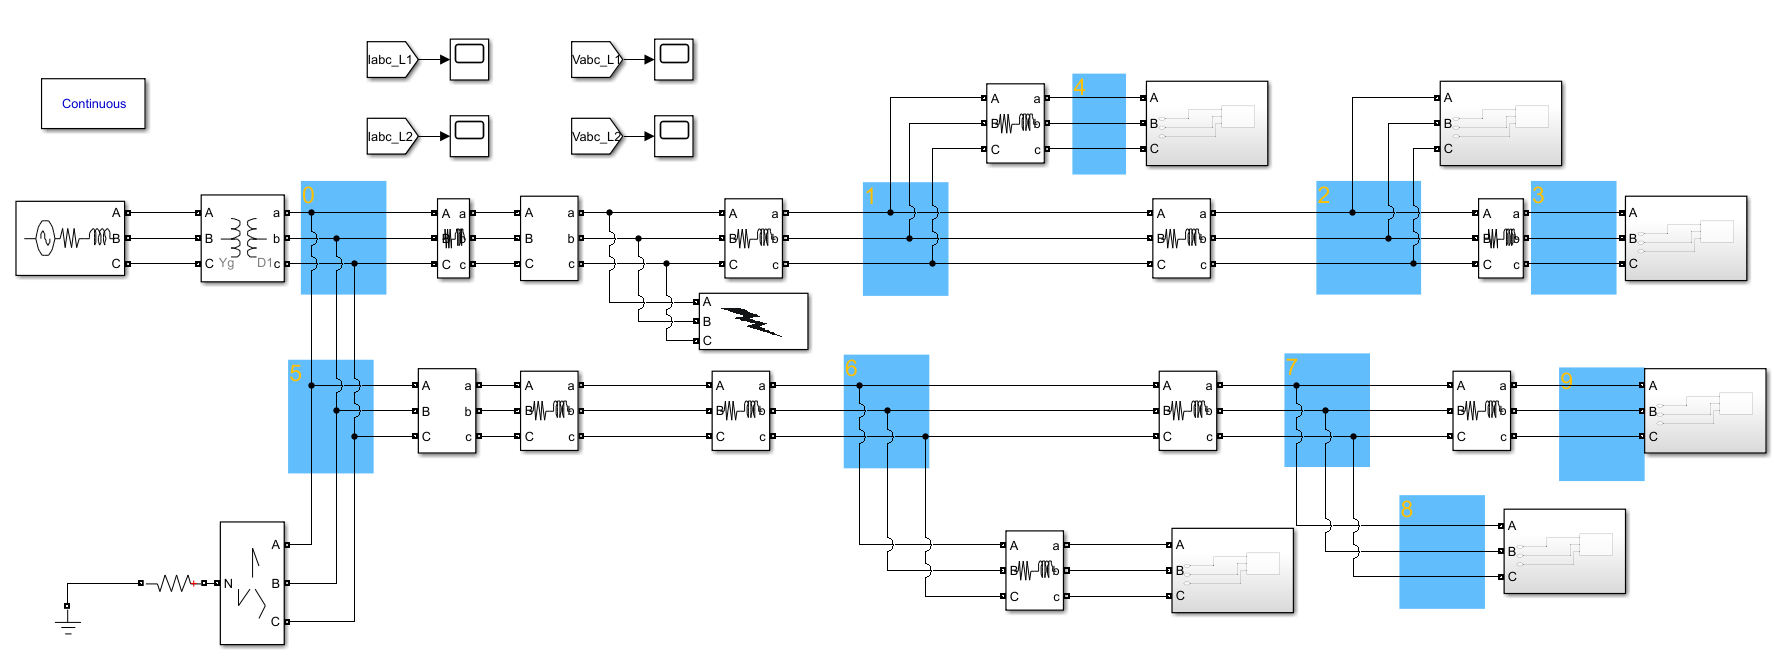
\includegraphics[width=13cm]{figure/1.png}
		\caption{基于Simulink的10kV小电阻接地系统的电磁暂态模型}
	\end{figure}

	其中,不同的注释方块表示原图中不同的结点。输电线路采用串联的电阻和电感表示,用单位阻抗值乘以距离表示不同的输电线长度。(这里不采用Distributed Parameters Line和Three-Phase PI Section Line模块的原因见下)
	
	Three-Phase Fault模块提供四种故障模型。按照论文中的仿真模拟顺序,通过比对结果是否一致,即可判断模型是否有误。然而,在仿真的时候,依次遇到了如下问题,花费了很多的时间,只解决了一部分,现归纳如下。
	
	\subsection{仿真时间太久}
	
	设定的仿真时间为0~0.5s,然而,在最初的模型中,需要经过将近两分钟才能模拟出结果。即使是在故障没有发生的0~0.1s内,示波器上绘制正常三相电流电压波形的速度仍然很慢。显然,这个模型并不算是特别复杂,这样的慢速是不正常的。
	
	因此,我先对模型进行了优化。发现,将Three-Phase PI Section Line替换为简单的阻抗模型后,模型的计算速度得到了很大的提升。为此,我认为是因为在simulink的计算中,Three-Phase PI Section Line模块由于考虑到了零序单位电阻、电容等其他效果的计算,导致总的计算量上升,降低了仿真速度。因此用串联的电阻和电感对输电线路进行简化,只考虑主要的影响。
	
	\subsection{波形震荡}
	
	当故障发生之后,波形除了表现出故障电流电压的特征外,还表现出了围绕故障电流电压曲线震荡。如下图:
	
	\begin{figure}[htpb]
		\centering
		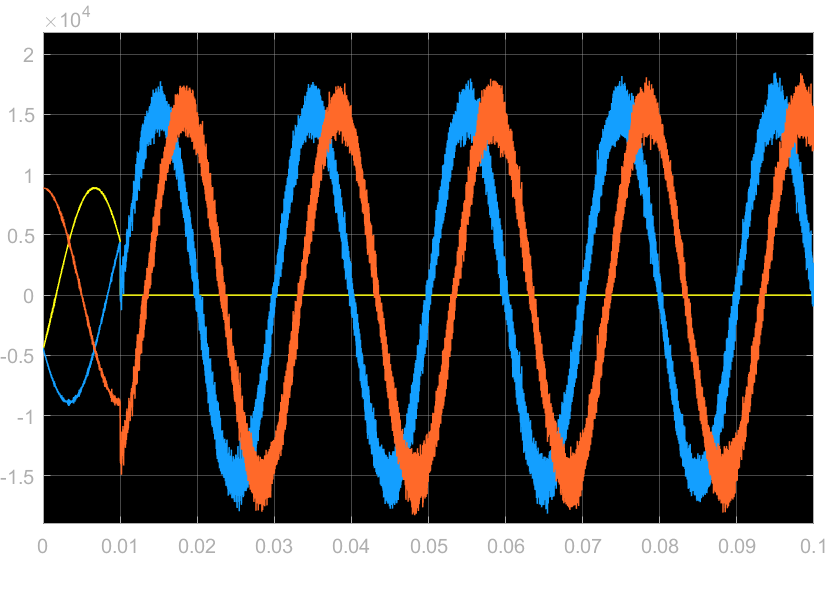
\includegraphics[width=7cm]{figure/2.png}
		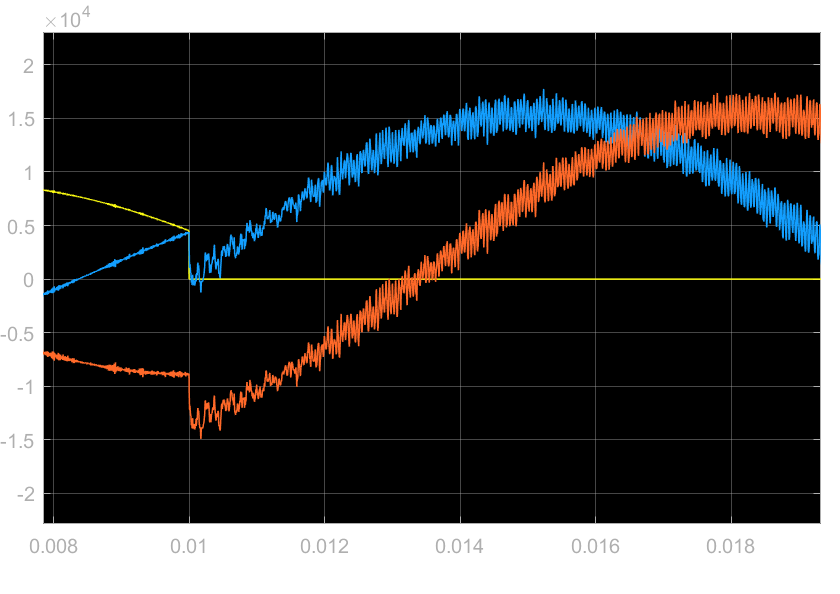
\includegraphics[width=7cm]{figure/3.png}
		\caption{曲线震荡}
	\end{figure}

	虽然图像的整体走向是没有问题的,但是显然这样的震荡是不正常的。起初,我认为是模型设定上有问题,调整了模块的参数,检查电路之后依旧无法解决。为此,我查阅了一些网上的论坛,最终发现问题出现在模型仿真步长的设定上。在采用ode23tb求解器时,由于仿真最大步长设置为自动,因此出现了这样的情况。在把求解器最大步长设置为1e-06之后,再次运行,波形的震荡消失。
	
	除此之外,我还尝试把求解最大步长分别调大和调小,发现步长调大之后计算时间下降,但是出现不同程度波形震荡的情况;步长调小之后,波形绘制速度减慢。这与感性的认知是一致的。
	
	针对这个问题,我主要的时间都花费在了解决波形震荡上面,包括上周模型中出现的比较崩溃的结果,都与其有关。甚至,在李戎学长的论文中,发现他的作图中对于正常的三相电流电压波形,也表现出了不规则正弦波的情况,在波顶处出现折线。这些都是求解步长的问题,而不是模型本身的问题。合理设置求解步长,在波形绘制精度和求解时间上做到平衡,对计算机仿真有重要的作用。属于比较刻骨铭心的收获。
	
	\subsection{仿真结果}
	
	在李戎学长给出的仿真结果和我的仿真结果比对的过程中,发现单相短路接地和两相短路接地时仿真结果基本一致。
	\begin{figure}[h]
		\centering
		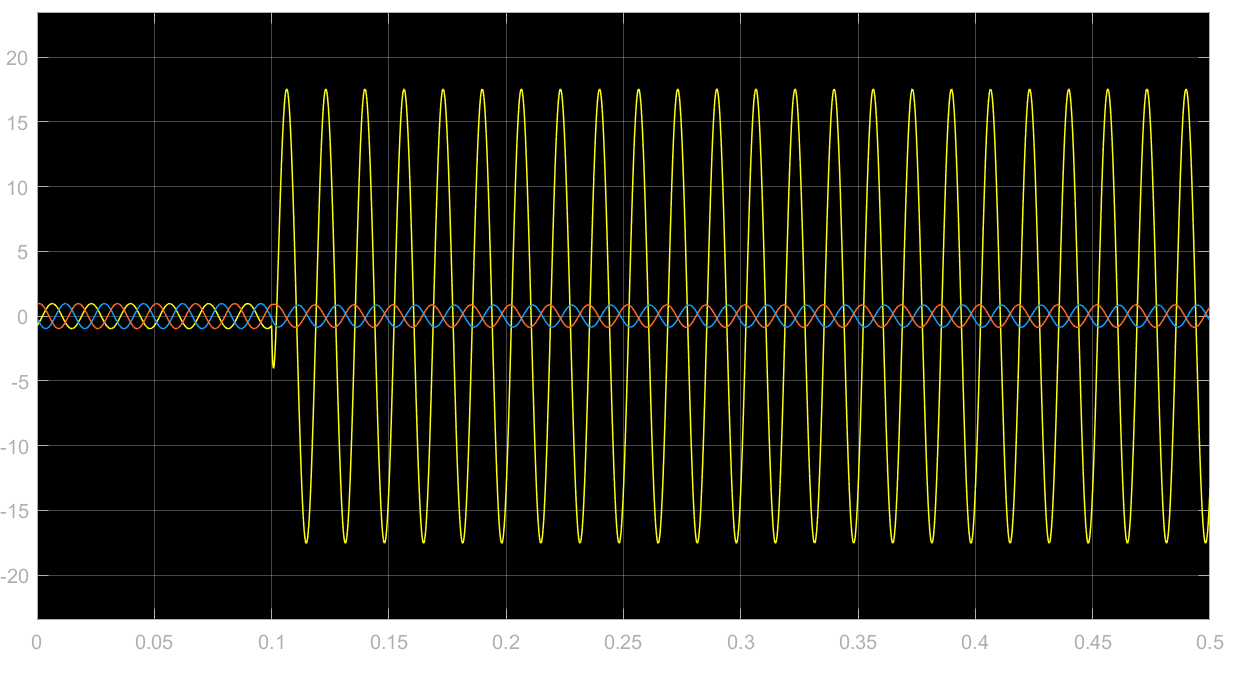
\includegraphics[width=6cm]{figure/4.png}
		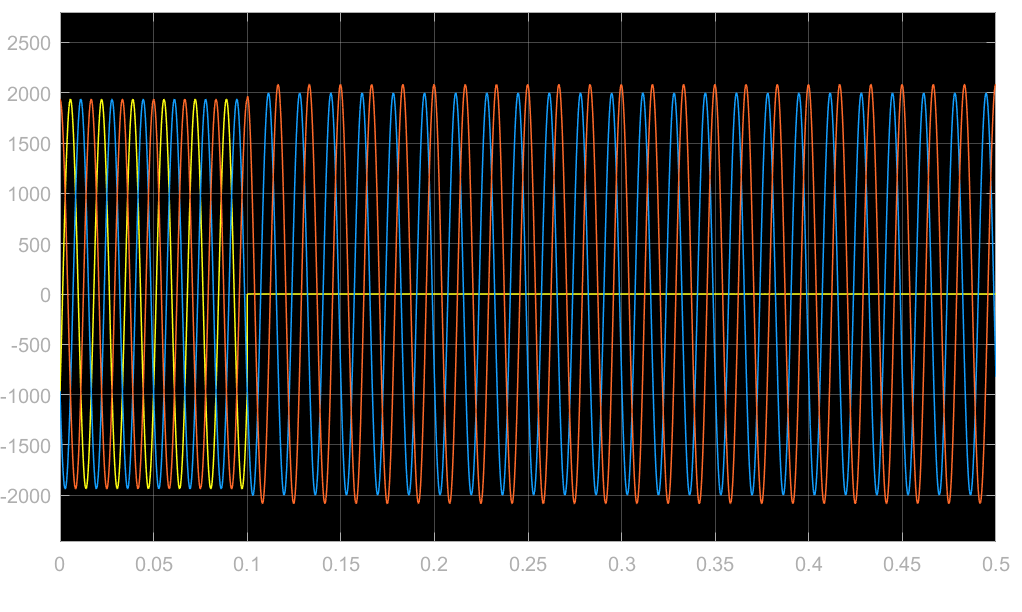
\includegraphics[width=6cm]{figure/5.png}
		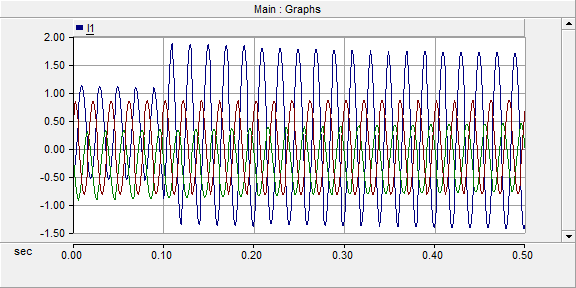
\includegraphics[width=6cm]{figure/6.png}
		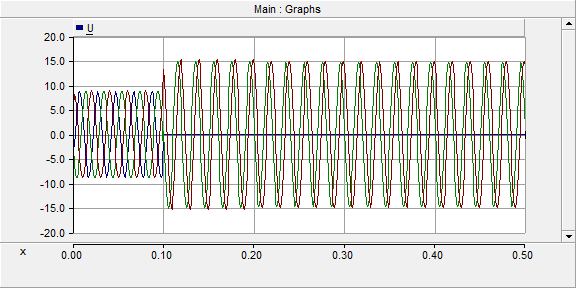
\includegraphics[width=6cm]{figure/7.png}
		\caption{距离0点100m处A相短路接地时馈线1的电流电压}
	\end{figure}
	\begin{figure}[h]
		\centering
		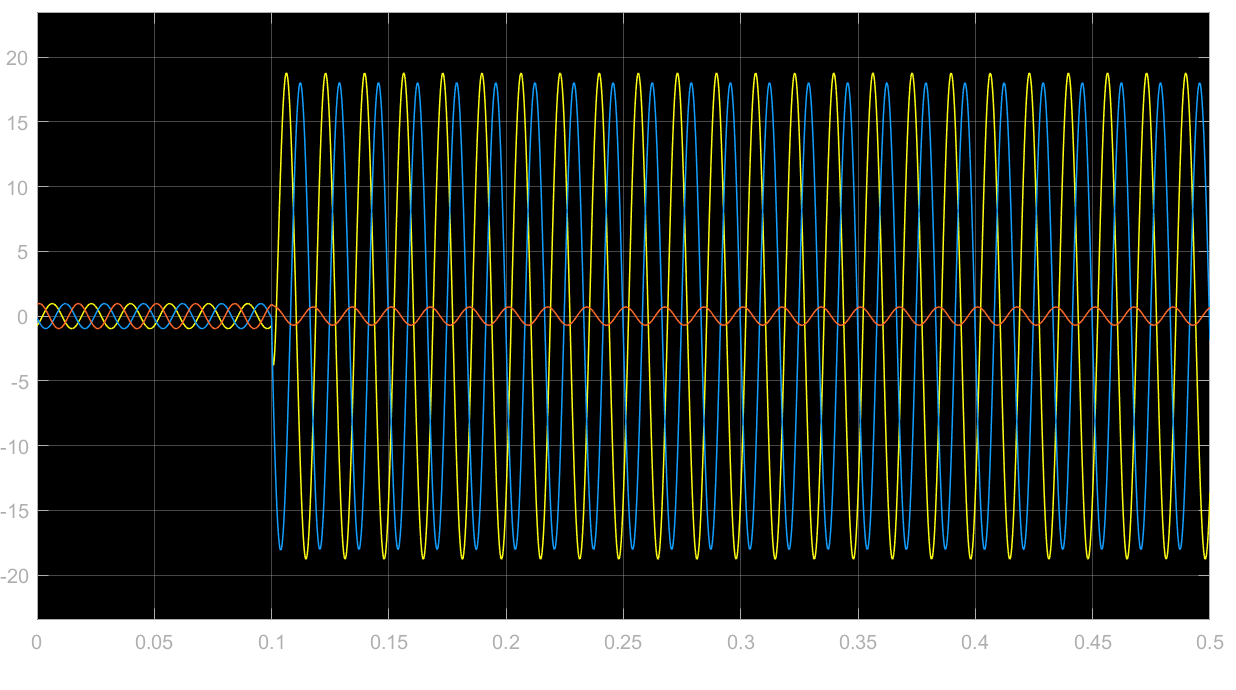
\includegraphics[width=6cm]{figure/8.png}
		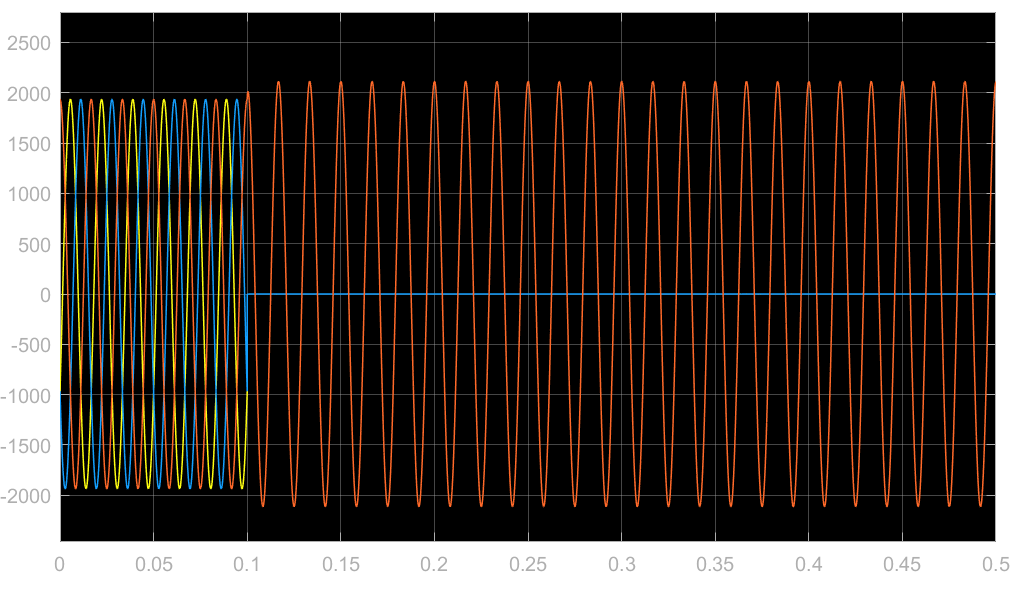
\includegraphics[width=6cm]{figure/9.png}
		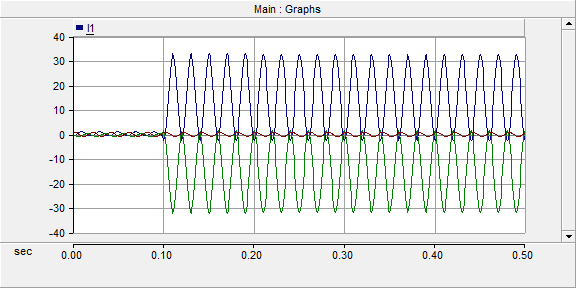
\includegraphics[width=6cm]{figure/10.png}
		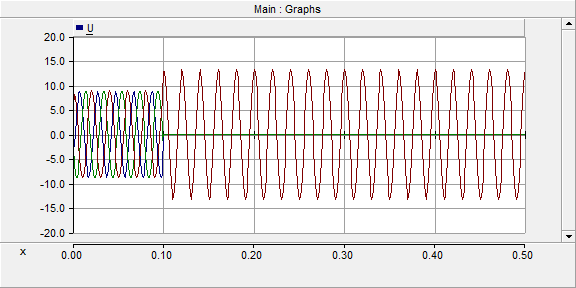
\includegraphics[width=6cm]{figure/11.png}
		\caption{距离0点100m处A、B相短路接地时馈线1的电流电压}
	\end{figure}

	除了波形的幅值不同,可能是由于具体的电路参数不同导致,但是波形的走向相同,说明模型没有问题。
	
	这里有一个细节是,距离0点100m处A、B相短路接地时馈线1的电流波形,在李戎学长的论文图中,AB相电流几乎只有正向和负向的值,而我的仿真图中出现了正负半周几乎等幅的情况,这是电路参数导致的问题吗?
	
	另外,我还发现李戎学长的图像中,在正常情况下三相电流不稳定,有幅值衰减的问题。这是因为什么,是由于求解的精度不够吗?
	
	\begin{figure}[H]
		\centering
		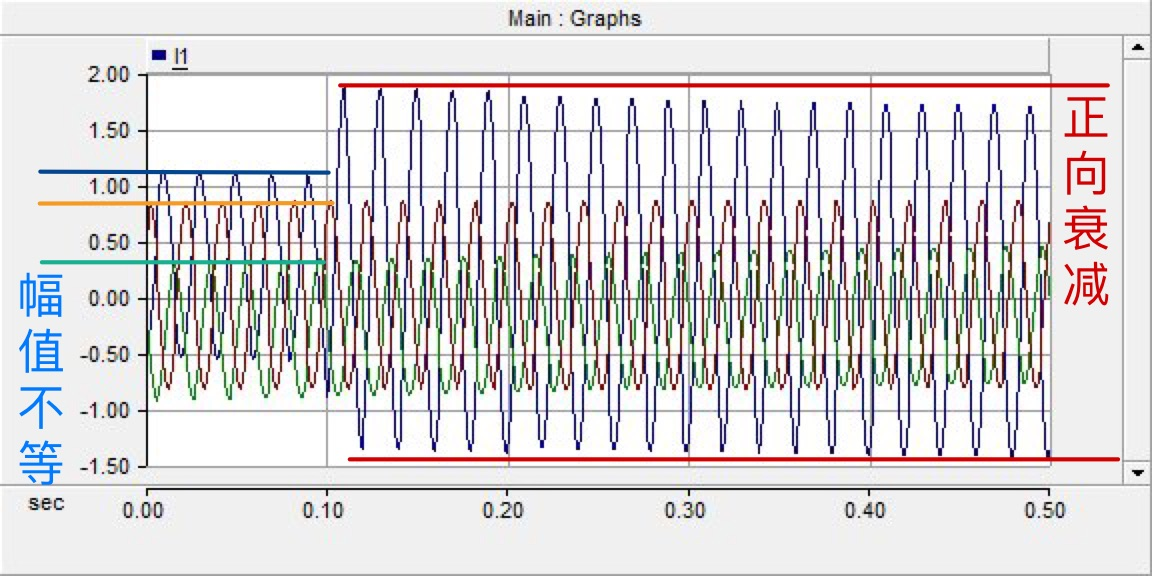
\includegraphics[width=7cm]{figure/6-1.jpg}
		\caption{幅值衰减与幅值不等}
	\end{figure}
	
	除此之外,我看到学长图中ABC三相即使是在正常的情况下,幅值也不相等。这个是由于什么因素造成的?是因为A、B、C相在负载端单独引出接了不同的负载吗,如果是,在模型中该如何体现。
	
	\section{利用MATLAB构建神经网络}
	
	由于论文中已经给出了神经网络的结构和参数,因此这一部分工作比较容易。有以下两点时遇到的问题:
	
	\begin{enumerate}
		\item 李教授对学长输入层结果的疑惑。确实论文在这一部分的叙述上不够详细。我的理解是输入层为一个imageInputLayer,大小为62*62,颜色通道为单通道,也就是说数据输入就是将故障发生后一段时间的波形转化成灰度图输入,不同的CNN都采用这样的输入,然而采用频率的确未知。
		\item 对于LRN归一层,在MATLAB中没有现成的命令指令可以生成,其具体实现方式还需要进行探索。
	\end{enumerate}

	因此,在下一周,需要将神经网络中LRN层实现构建,然后利用生成的样本数据集进行训练学习即可。在生成数据集的过程中,确实利用simulink不是很好的方案。我对PSCAD的下载进行了一下了解,想问一下李教授我们学校是否有购买PSCAD,如果过没有,我就自己想办法下载一个。
	
\end{document}